\documentclass[compress]{beamer}
\usepackage[utf8]{inputenc}
\usepackage{natbib,amsmath,calc,amssymb,graphicx,tabularx,xr,multirow,times,enumitem,array}
%\usepackage[T1]{fontenc}
%\usepackage{default}
\usepackage{hyperref}
\usetheme{Singapore}
% \usecolortheme{beetle}
\definecolor{anthracite}{RGB}{0,0,0}
\definecolor{grey}{RGB}{150,150,150}
\setbeamercolor{background canvas}{bg=anthracite, fg=white}
\setbeamercolor{background}{fg=white, bg=anthracite}
\setbeamercolor{frametitle}{bg=anthracite,fg=white}
\setbeamercolor{title}{fg=white, bg=anthracite}
\setbeamercolor{normal text}{fg=white,bg=anthracite}

% \setbeamercolor{palette primary}{fg=white, bg=anthracite}
% \setbeamercolor{palette secondary}{fg=white, bg=anthracite}
% \setbeamercolor{palette tertiary}{fg=white, bg=anthracite}
% \setbeamercolor{palette quaternary}{fg=white, bg=anthracite}
\setbeamercolor{local structure}{fg=white, bg=anthracite}
\setbeamercolor{structure}{fg=white, bg=grey}
\setbeamercolor{section in head/foot}{fg=white, bg=anthracite}

\usepackage[T1]{fontenc}


%add the little bullets for the slides
\useoutertheme{miniframes}
\usepackage{etoolbox}
% \usepackage{enumitem}
\usepackage{multimedia}
\makeatletter

%%%%
%%%% THIS MAKES SOME NAVIGATION CYRCLES DISAPPEAR BY USING THE COMMANDS \miniframesoff or \miniframeson : useful for skipping title slide or when 
%there are too many slides
%%%%
\useoutertheme[subsection=false]{miniframes}
\let\beamer@writeslidentry@miniframeson=\beamer@writeslidentry
\def\beamer@writeslidentry@miniframesoff{%
  \expandafter\beamer@ifempty\expandafter{\beamer@framestartpage}{}% does not happen normally
  {%else
    % removed \addtocontents commands
    \clearpage\beamer@notesactions%
  }
}
\newcommand*{\miniframeson}{\let\beamer@writeslidentry=\beamer@writeslidentry@miniframeson}
\newcommand*{\miniframesoff}{\let\beamer@writeslidentry=\beamer@writeslidentry@miniframesoff}
%%%
%%%

%% essential for showing the bullets!!
\usepackage{remreset}
\@removefromreset{subsection}{section}
\setcounter{subsection}{1}
%%

\setbeamertemplate{navigation symbols}{}

\makeatother


\begin{document}

 \section{Discussion}

\begin{frame}
\frametitle{Single cell vs multiple cells}
\begin{itemize}
 \item Perstime: how straight or wiggly
 \item Few cells, no adhesion: random walk
 \item More cells and/or adhesion: streaming
\end{itemize}

\end{frame}


\begin{frame}
\frametitle{Using active migration with adhesion}
Get closer to minimal energy configuration: break through local optima.
\begin{center}
 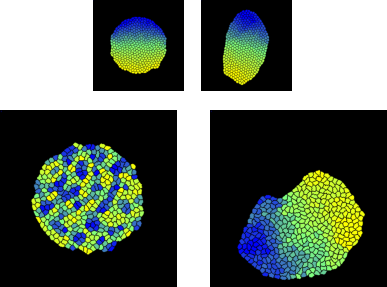
\includegraphics[width=0.8\textwidth]{figures/gradedadhesion2.pdf}\\
\end{center}
\end{frame}


\section{T cells in lymph nodes}
%Hold court on tcells circulating through blood and lymph nodes, Lymph nodes are hubs where they find antigen-presenting cells and get activating signals
\begin{frame} 
\frametitle{T cells need to be activated}   
\begin{center}
 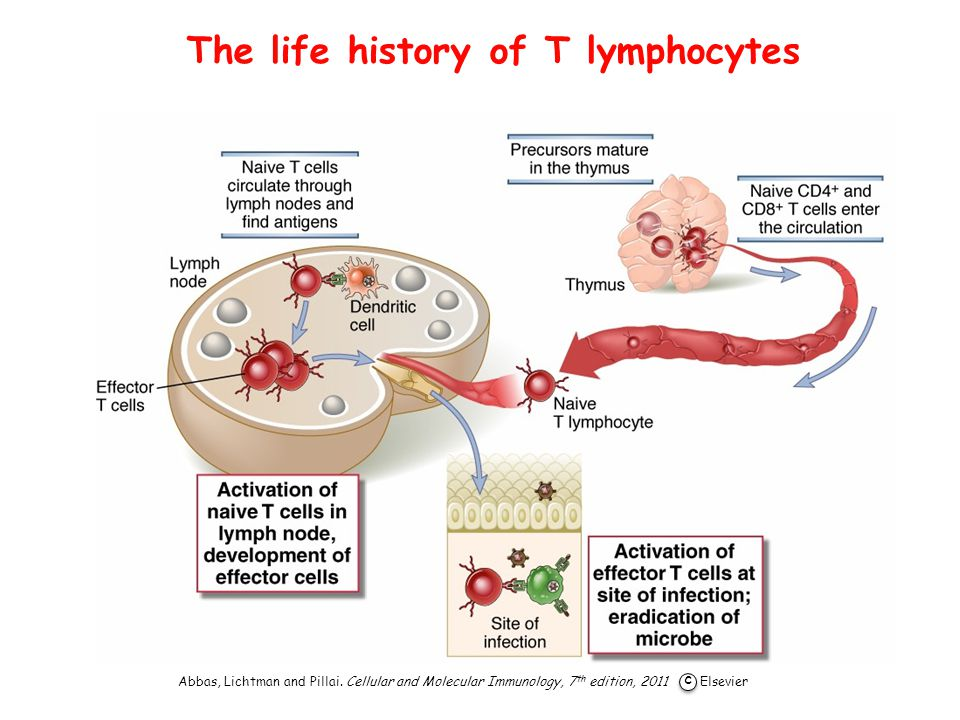
\includegraphics[width=0.8\textwidth]{figures/tcellcycle.jpg}\\
\end{center}
\end{frame}

\begin{frame} 
\frametitle{T cell migration}   
\begin{center}
 \movie[width=7cm, height=7cm, poster, loop]{}{joost_tcells2p.mpg} \\
\end{center}
\end{frame}

\begin{frame} 
\frametitle{Lymph nodes are very packed}   
\begin{center}
\movie[width=7cm, height=7cm, poster, loop]{}{joost_ret.mpg} \\
\tiny Beltman \textit{et al.} 2007
\end{center}
\end{frame}

\begin{frame}
\frametitle{Lymph node structure causes realistic migration}   
\begin{center}
\movie[width=5cm, height=5cm, poster, loop]{}{joost_streams.mpg} 
\movie[width=5cm, height=5cm, poster, loop]{}{joost_proj.mpg} 
\tiny Beltman \textit{et al.} 2007
\end{center}
\end{frame}

\begin{frame}
\frametitle{A T cell's perspective}   
\begin{center}
\movie[width=7cm, height=7cm, poster, loop]{}{joost_roller.mpg} 
\tiny Beltman \textit{et al.} 2007
\end{center}
\end{frame}

\begin{frame}
\frametitle{Another application in immunology} %CPM is the bestest
Before immune response is mounted, fraction of antigen-specific T cells is ~$10^{-5},10^{-6}$\\ 
How does an antigen-presenting cell ``find'' the right T cell? It's the T cells that move.
Chemotaxis? %not going to explain how chemotaxis works
\begin{center}
 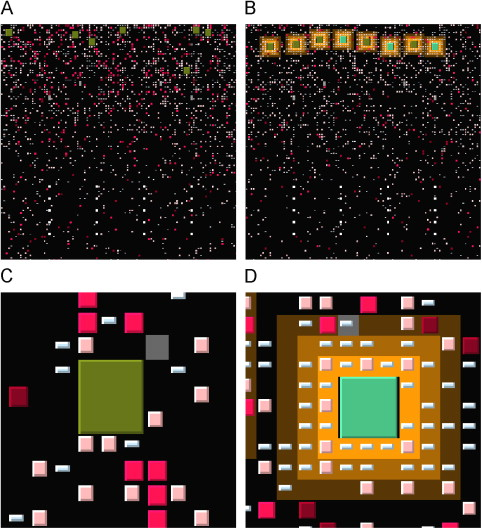
\includegraphics[width=0.5\textwidth]{figures/riggs.jpg}\\
 \tiny Riggs \textit{et al.,} 2008
\end{center}
\end{frame}

\begin{frame}
\frametitle{Model without chemotaxis} %CPM is the bestest
\begin{center}
\movie[width=7cm, height=7cm, poster, loop]{}{VideoS1.mp4} 
\end{center}
\end{frame}

\begin{frame}
\frametitle{Chemotaxis does help} %CPM is the bestest
\begin{center}
\movie[width=7cm, height=7cm, poster, loop]{}{VideoS2.mp4} 
\end{center}
...so long as cells do not get crushed
\end{frame}

\begin{frame}
\frametitle{Another way to implement cell migration}   
\begin{center}
 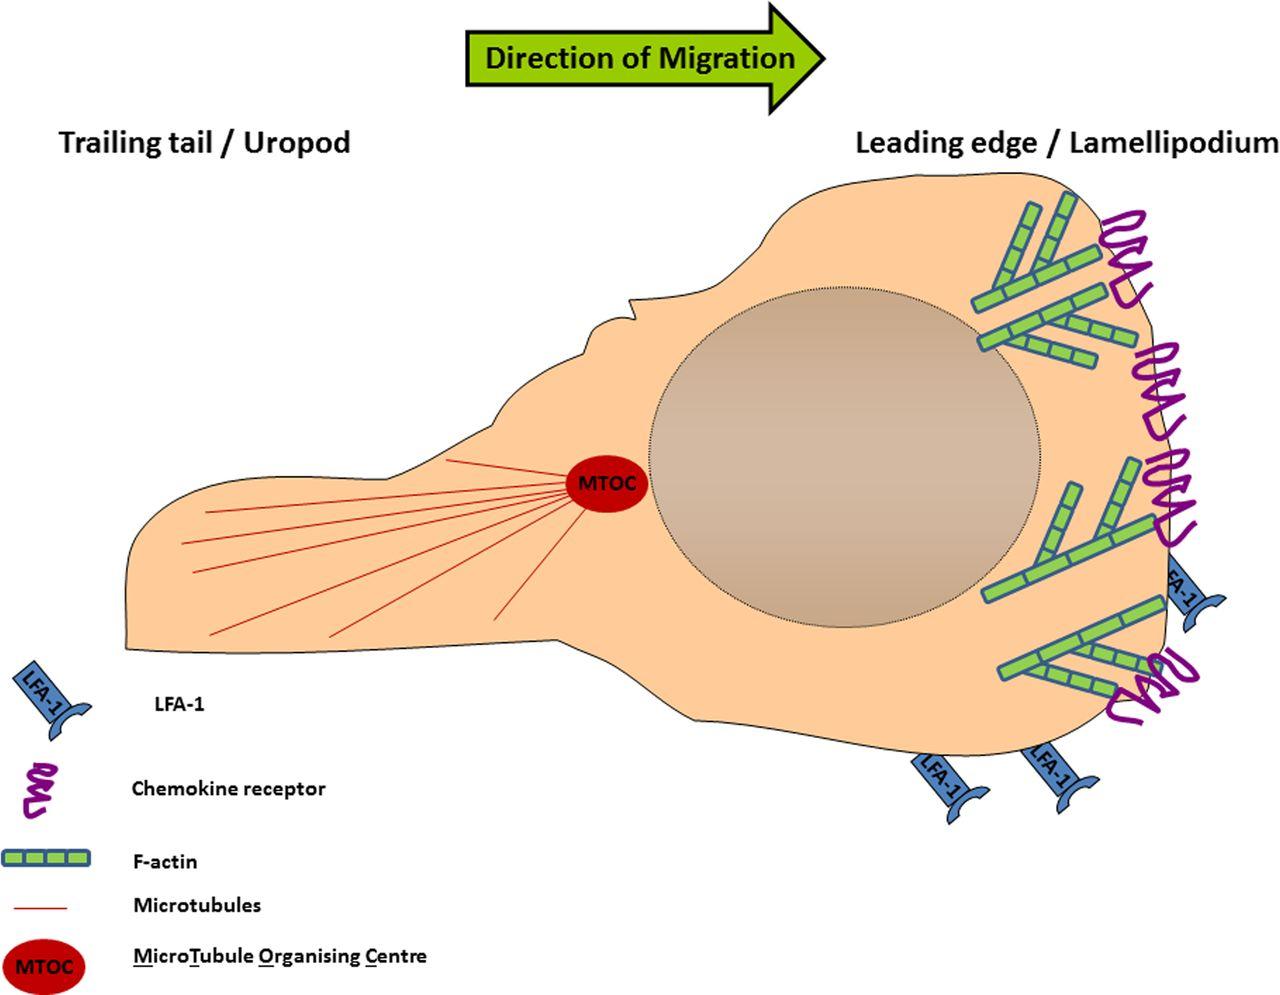
\includegraphics[width=0.5\textwidth]{figures/actinmigration.jpg}\\
 \tiny Niculescu \textit{et al.,} 2015
\end{center}

\end{frame}

\begin{frame}
\frametitle{Another way to implement cell migration}   
\begin{center}
 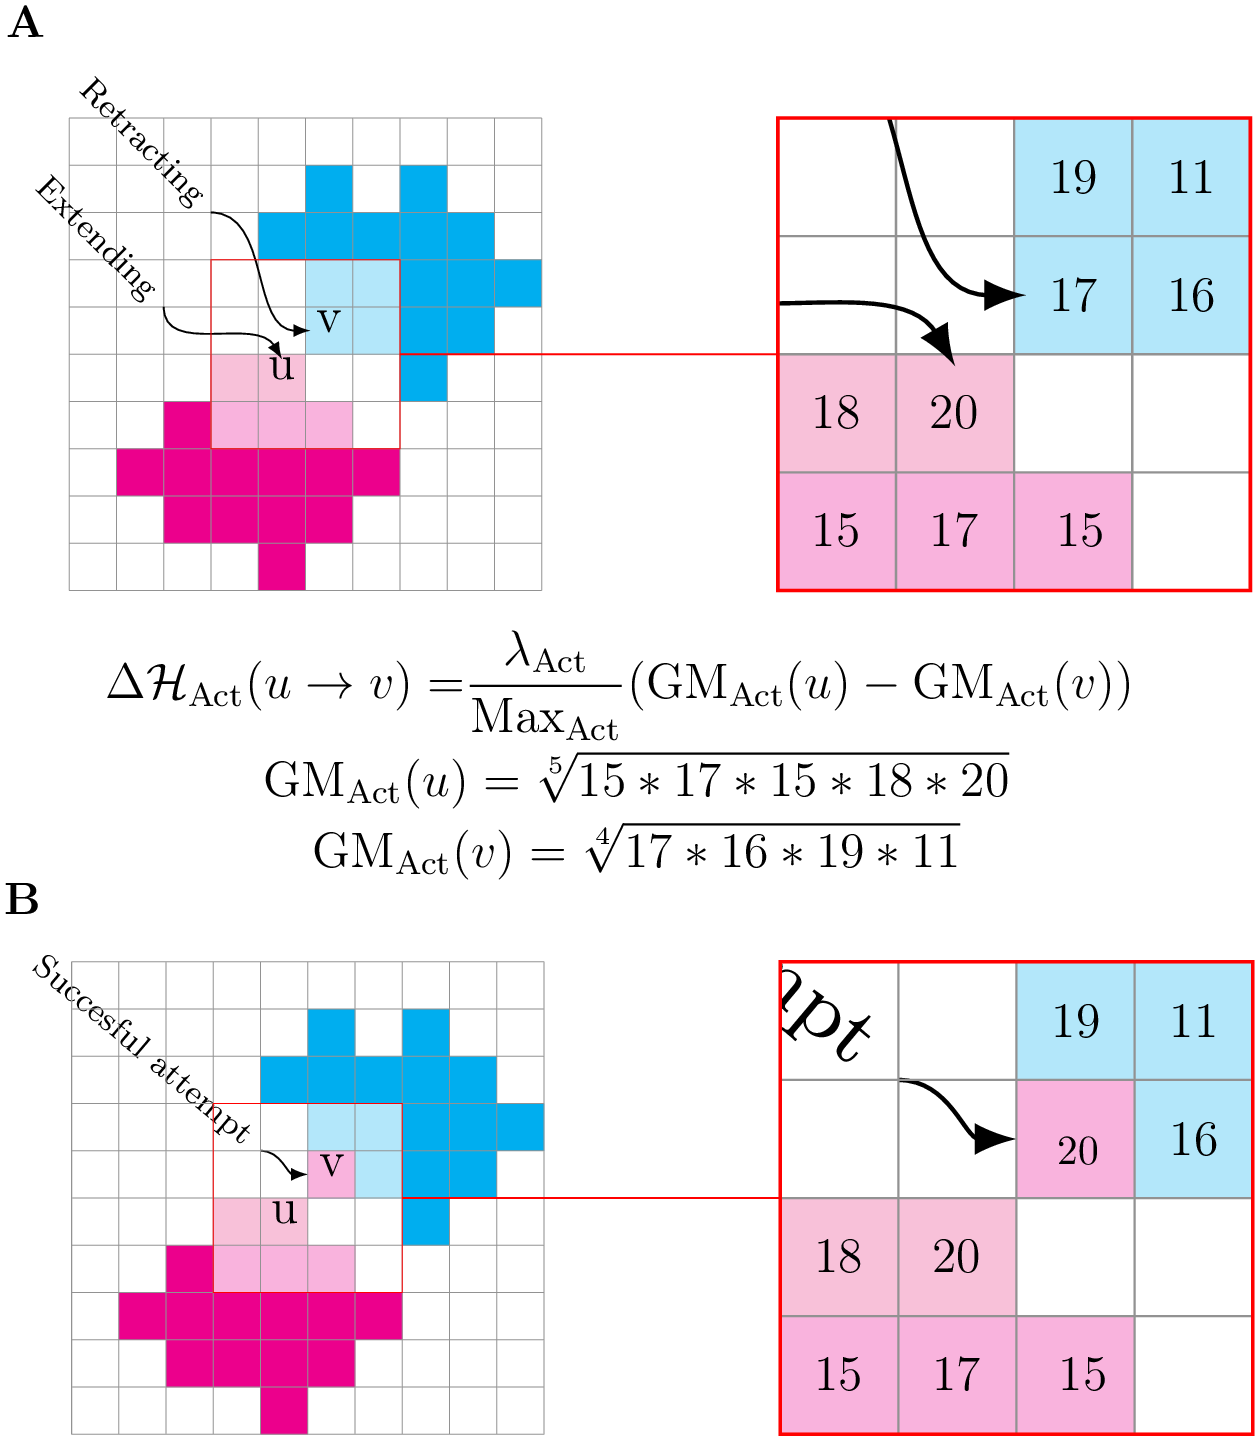
\includegraphics[width=0.5\textwidth]{figures/ioana_model.png}\\
 \tiny Niculescu \textit{et al.,} 2015
\end{center}

\end{frame}

\begin{frame}
\frametitle{two main modes} %CPM is the bestest
\begin{center}
 Amoeboid ~~~~~~~~ keratocyte-like
\end{center}

\movie[width=5cm, height=5cm, poster, loop]{}{polarisation_amoeboid_annotated.mp4} 
\movie[width=5cm, height=5cm, poster, loop]{}{polarisation_kera_annotated.mp4} 
\end{frame}

\begin{frame}
\frametitle{multiple modes of migration possible} %CPM is the bestest
\movie[width=7cm, height=7cm, poster, loop]{}{morphospace_lossless.mp4} 
\end{frame}

\begin{frame}
\frametitle{Tissue context makes migration pattern} %CPM is the bestest
\begin{center}
\movie[width=6.5cm, height=6.5cm, poster, loop]{}{skin.mpg} 
\end{center}
\small Amoeboid cells are better able to squeeze through tightly packed tissue\\
\end{frame}

\section{Moving to EvoDevo}
\begin{frame}
\frametitle{Endless forms most beautiful...}   
\begin{itemize}
 \item Cell growth, cell death: increase target volume or set to 0
 \item Cell division or cleavage: Assign new ID to part of the cell
 \item Chemotaxis: $\Delta H += \mu_{chem}(C_{neigh}-C_{target})$
 \item Cortical tension: surface area constraint = $H += \lambda_{s}(s-S)^2$
 \item Cell elongation (various ways)
 \item different J values along parts of membrane
 \item elastic springs between cells
 \item secretion of signalling molecules or ECM
 \item Gene expression (influencing any cell property)
\end{itemize}
\end{frame}

\begin{frame}
\frametitle{Platforms}   
\begin{center}
\begin{itemize}
 \item CompuCell3D
 \item Morpheus
 \item Tissue Simulator
 \item Chaste
\end{itemize}

\end{center}

\end{frame}

\begin{frame}
\frametitle{...have been, and are being, evolved}   
\begin{center}
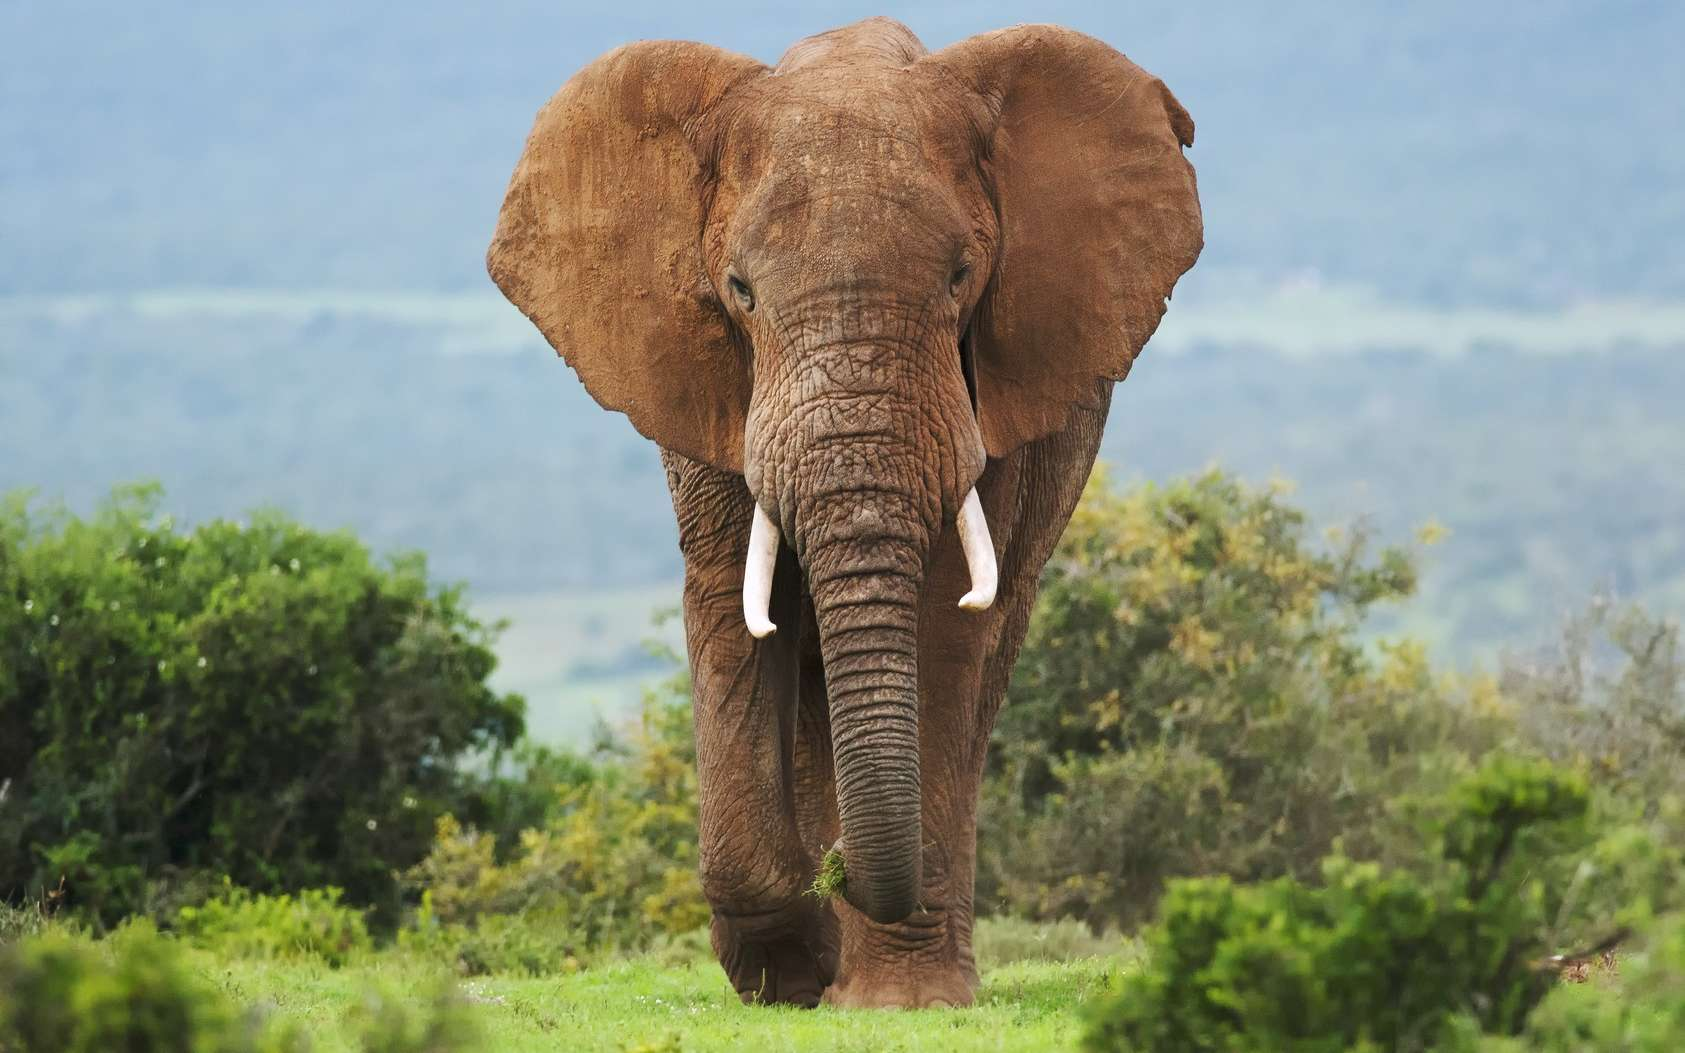
\includegraphics[width=0.75\textwidth]{figures/elephant.jpg} 
\end{center}

Ernst Mayr

\end{frame}

\begin{frame}
\frametitle{The signature of evolution}   

\begin{center}
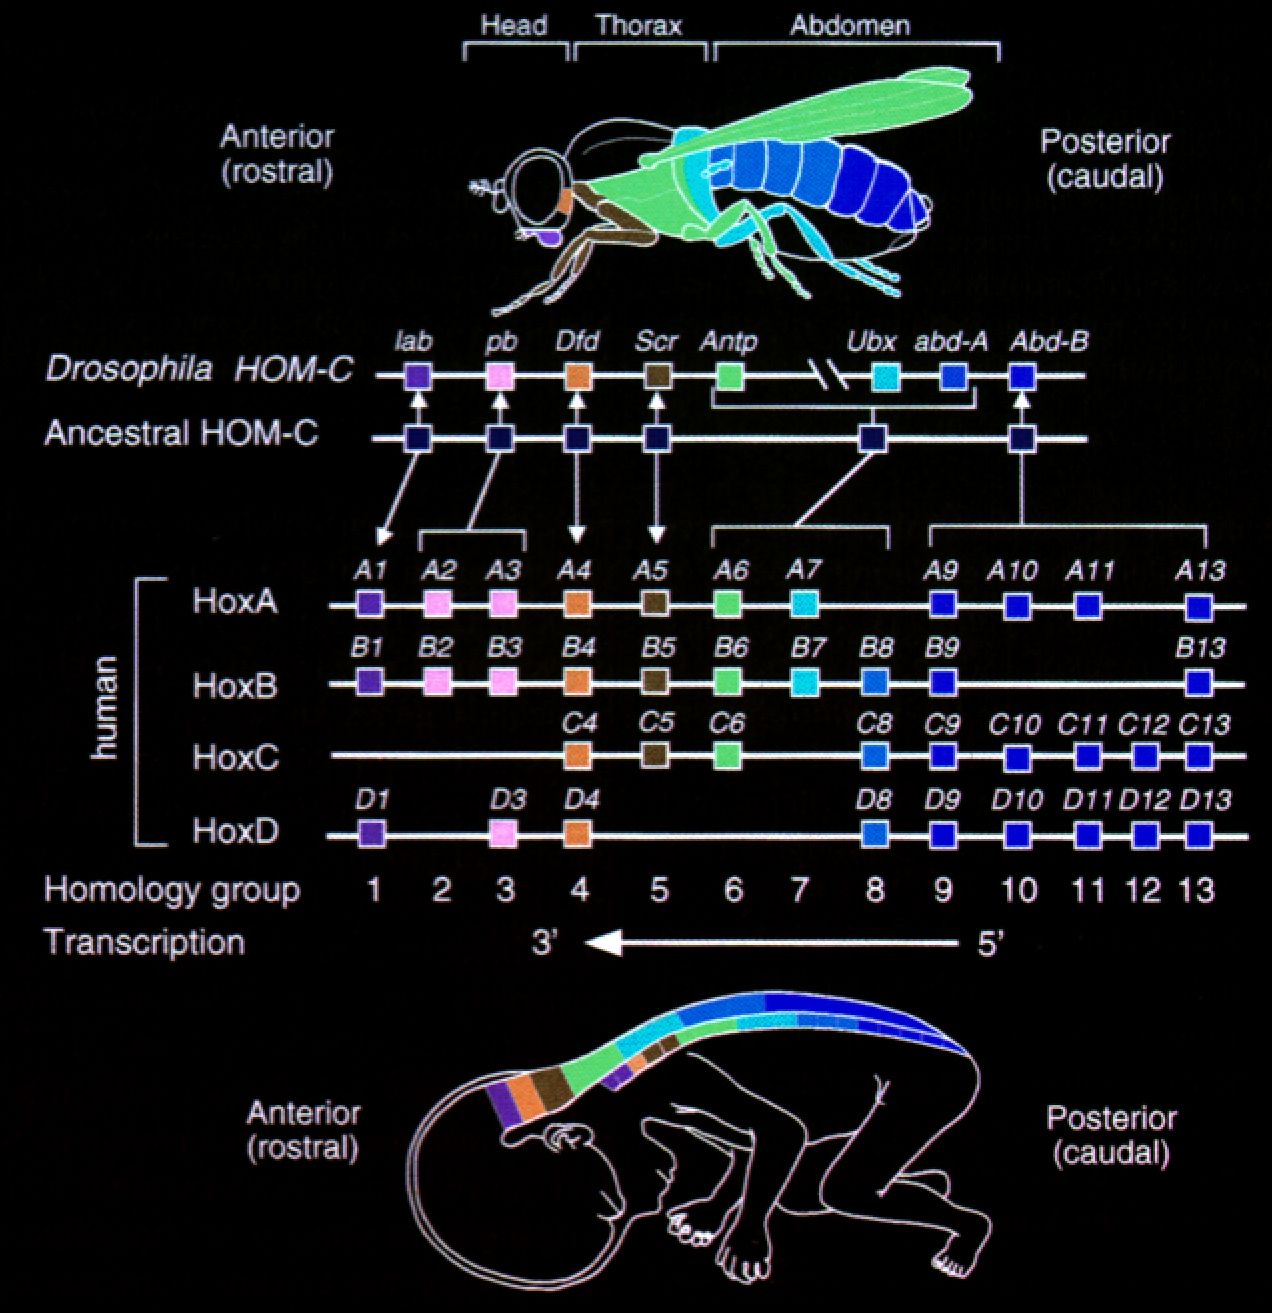
\includegraphics[width=0.6\textwidth]{figures/evodevo.jpg} 
\end{center}

\end{frame}


\begin{frame}
\frametitle{The importance of the GP map}   

From the genotype to the phenotype:\\ a long and complex path
\begin{center}
\includegraphics[width=0.95\textwidth]{figures/scales.pdf} 
\end{center}

Feedback between different levels, also for development
\end{frame}

\begin{frame}
\frametitle{The questions of Evo-Devo}   

Why do we see certain developmental mechanisms?\\
How do developmental mechanisms shape future evolution, and vice versa?

\end{frame}

\section{Animal segmentation}
\begin{frame}
    \frametitle{Clades with segmentation}
    % insert pretty picture with segments
    \begin{center}
    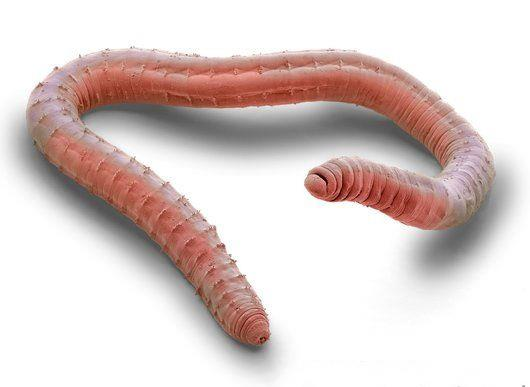
\includegraphics[width=0.35\textwidth]{figures/annelid_SEM.jpg}
    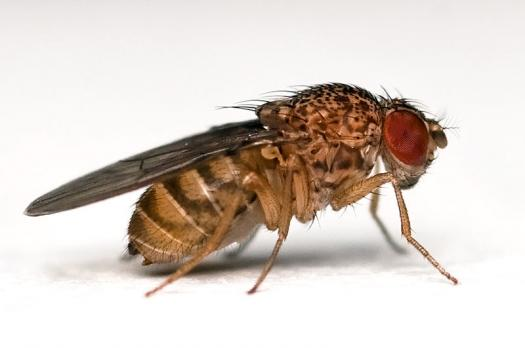
\includegraphics[width=0.35\textwidth]{figures/drosophila.jpg}
    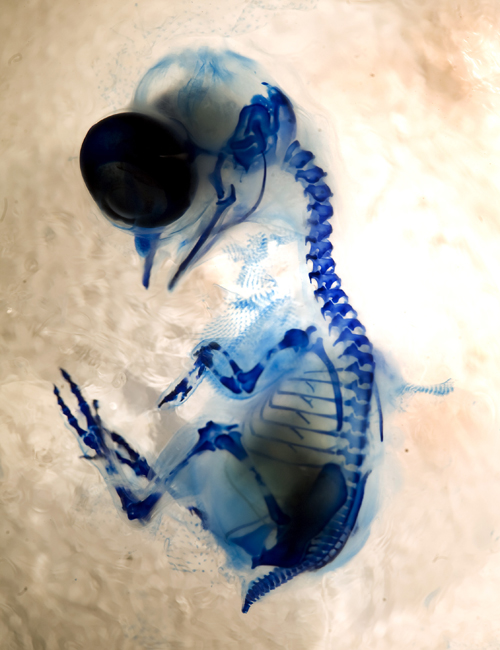
\includegraphics[width=0.35\textwidth]{figures/chick_vertebrae.jpg}
    \\~\\
    \end{center}
   % Here I show the three prominent clades which are segmented: arthropods, annelids and vertebrates.
  \end{frame}

\begin{frame}
    \frametitle{Segmentation across bilateria}
    % insert pretty picture with segments
   \begin{center}
     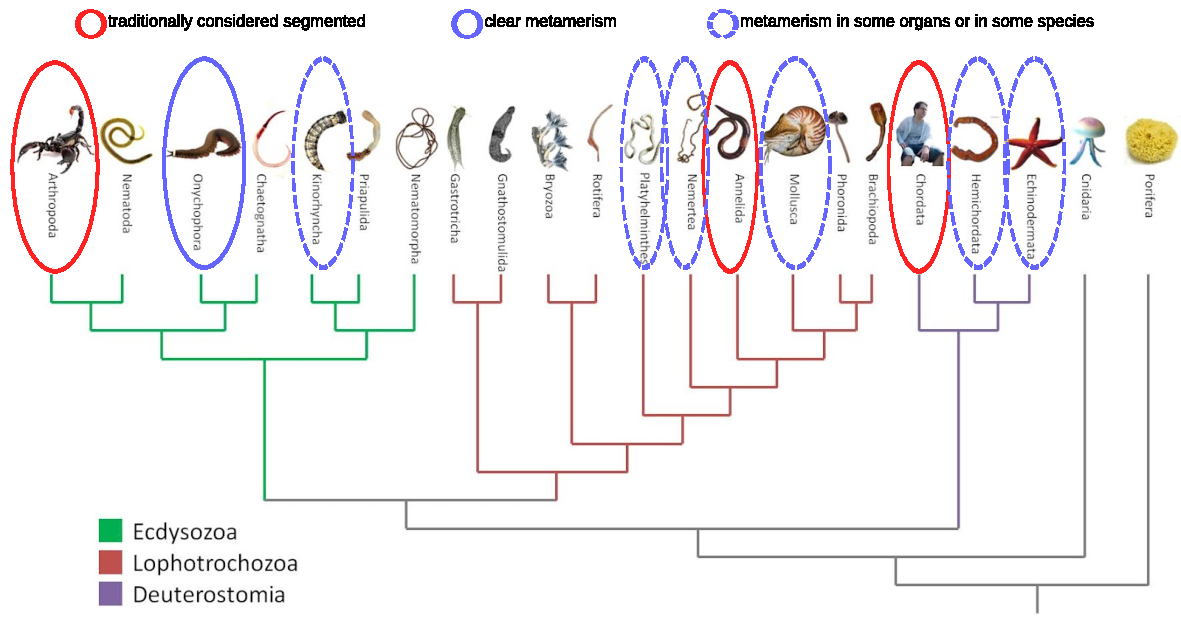
\includegraphics[width=0.9\textwidth]{figures/tree_animals.pdf}
     \\~\\
   \end{center}
   three overtly segmented clades, others partially or pseudosegmented.
\end{frame}

\begin{frame}
\frametitle{Segmentation across bilateria}
    % insert pretty picture with segments
   \begin{center}
   sequential vs hierarchical
   \begin{columns}
    \begin{column}{0.48\textwidth}
     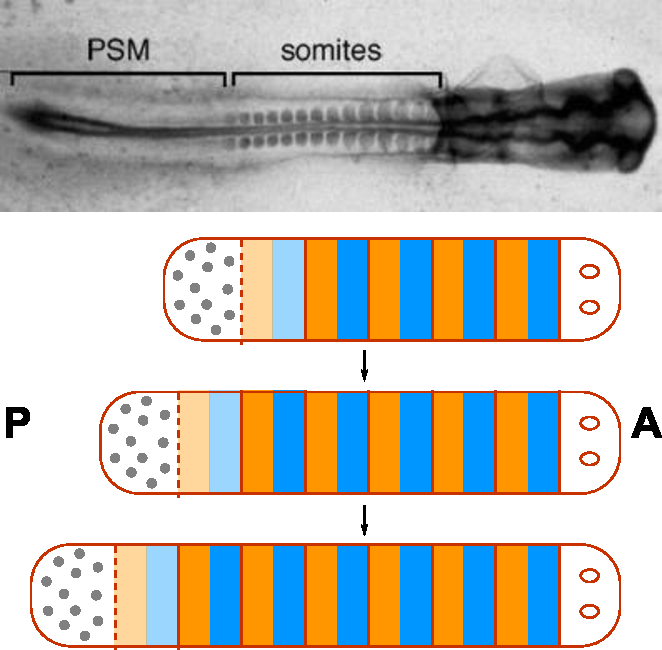
\includegraphics[width=0.9\textwidth]{figures/vertebrate_segmentation.pdf}
    \end{column}
    \begin{column}{0.48\textwidth}
     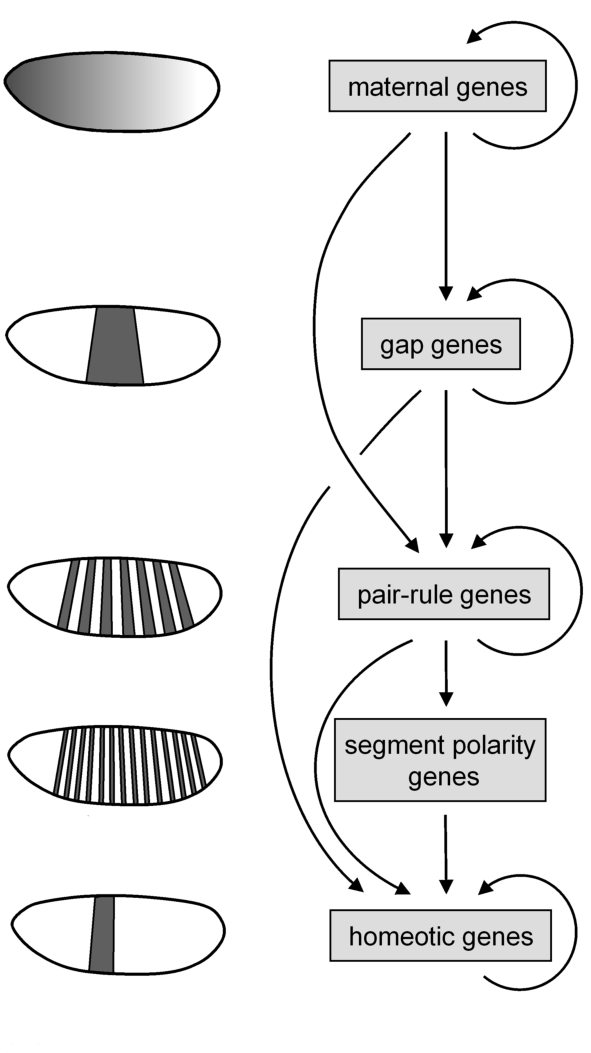
\includegraphics[width=0.6\textwidth]{figures/drosophila_hierarchy.pdf}
    \end{column}
   \end{columns}
   sequential is the more prevalent mechanism
    \end{center}
\end{frame}
\begin{frame}
    \frametitle{Vertebrates: clock and wavefront mechanism}
    % insert pretty picture with segments
   \begin{center}

     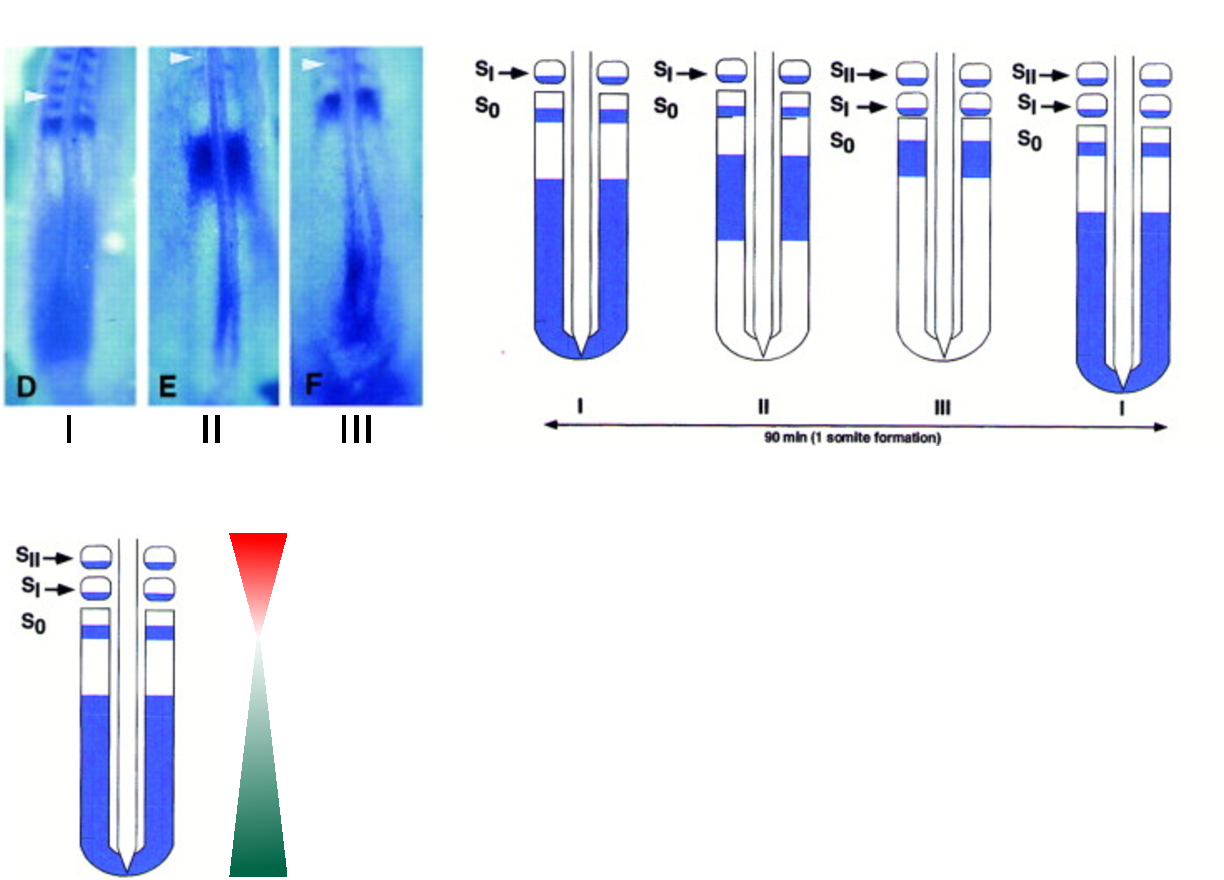
\includegraphics[width=0.75\textwidth]{figures/palmeirim_osc.pdf}\\
   % \\~\\
  
    \end{center}
{\bf clock:} gene expression oscillations\\
{\bf wavefront:} morphogen gradient due to local production and global decay
    % mechanism recently called into question
   % explain about transcription factors
\end{frame}
\begin{frame}
\frametitle{Resulting GRN dynamics}
   \begin{center}
\movie[width=0.6\textwidth,label=show3,poster, loop]{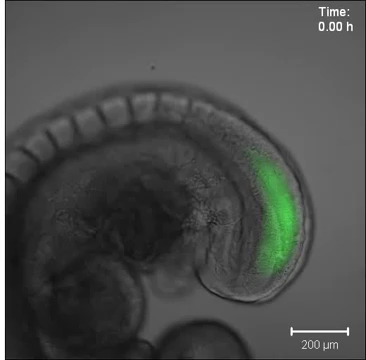
\includegraphics[width=0.6\textwidth]{figures/placeholder_wave.png}}{lfng_osc.mp4}\\    
   \end{center}

\end{frame}

\begin{frame}
    \frametitle{Segment development in insects}
    % insert pretty picture with segments
   \begin{center}
     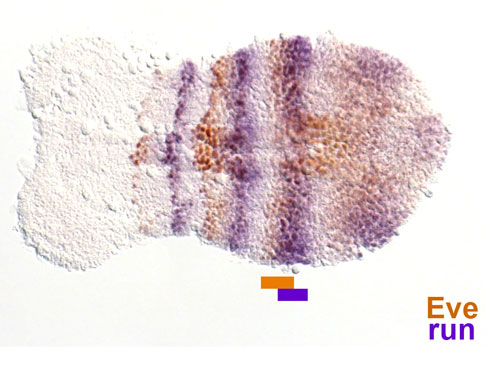
\includegraphics[width=0.5\textwidth]{figures/tribolium_eve_run.jpg}\\

    {\small Choe et al., 2006}
    \end{center}
    Evidence for a clock, nature of wavefront is unclear
   % explain about transcription factors
\end{frame}

\begin{frame}
    \frametitle{What do we want to know?}
    % insert pretty picture with segments
    \begin{center}
    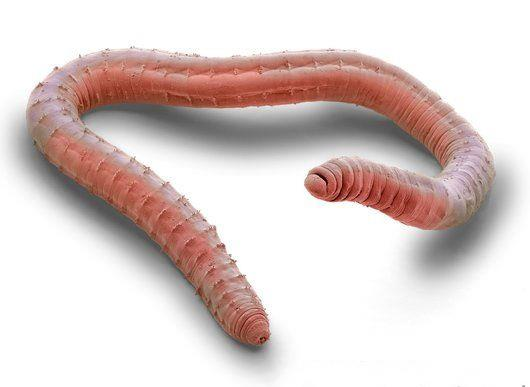
\includegraphics[width=0.3\textwidth]{figures/annelid_SEM.jpg}
    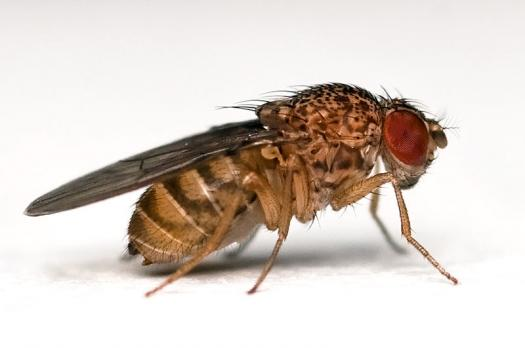
\includegraphics[width=0.3\textwidth]{figures/drosophila.jpg}
    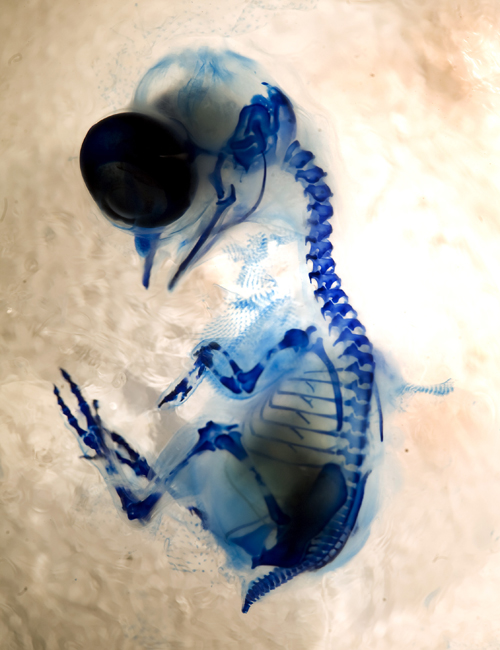
\includegraphics[width=0.3\textwidth]{figures/chick_vertebrae.jpg}
    \\~\\
    \end{center}
    
    \begin{itemize}
    \item Why the clock-and-wavefront mechanism?
    \item Can we understand the differences between vertebrates and insects?
    \item evolutionary origins of segmentation: what shaped the tree? %mention shared ancestry
    \end{itemize}

\end{frame}

\begin{frame}
    \frametitle{The likelihood of evolving sequential segmentation}
    \begin{center}
     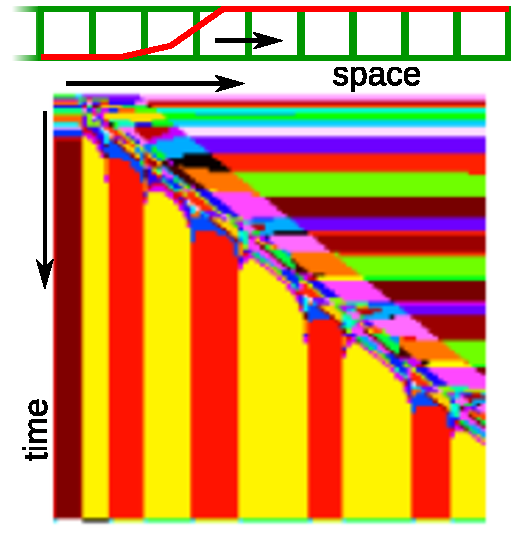
\includegraphics[width=0.6\textwidth]{figures/kirsten_model.pdf}\\
    {\small adapted from Ten Tusscher and Hogeweg, 2011}
    \end{center}
    % previous models have shown that seq. seg is likely to evolve in the presence of a movign wavefront
    % need to test this when axial growth has to evolve.
 \end{frame} 

\begin{frame}
    \frametitle{The likelihood of evolving sequential segmentation}
    \begin{center}
     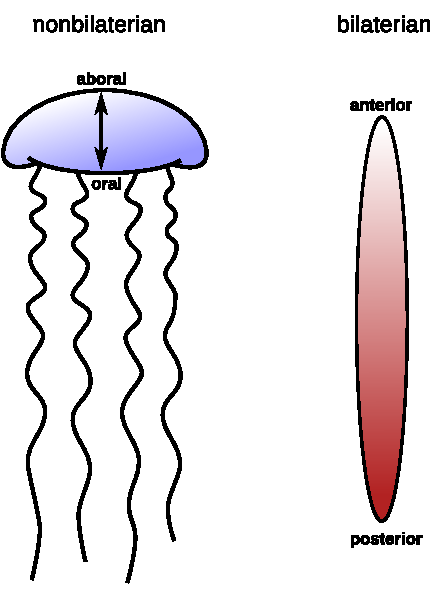
\includegraphics[width=0.5\textwidth]{figures/body_axis_change.pdf}\\
    \end{center}
    % previous models have shown that seq. seg is likely to evolve in the presence of a movign wavefront
    % need to test this when axial growth has to evolve.
 \end{frame} 
 
\begin{frame}
    \frametitle{Model of evolving and developing individuals}
    \begin{center}
     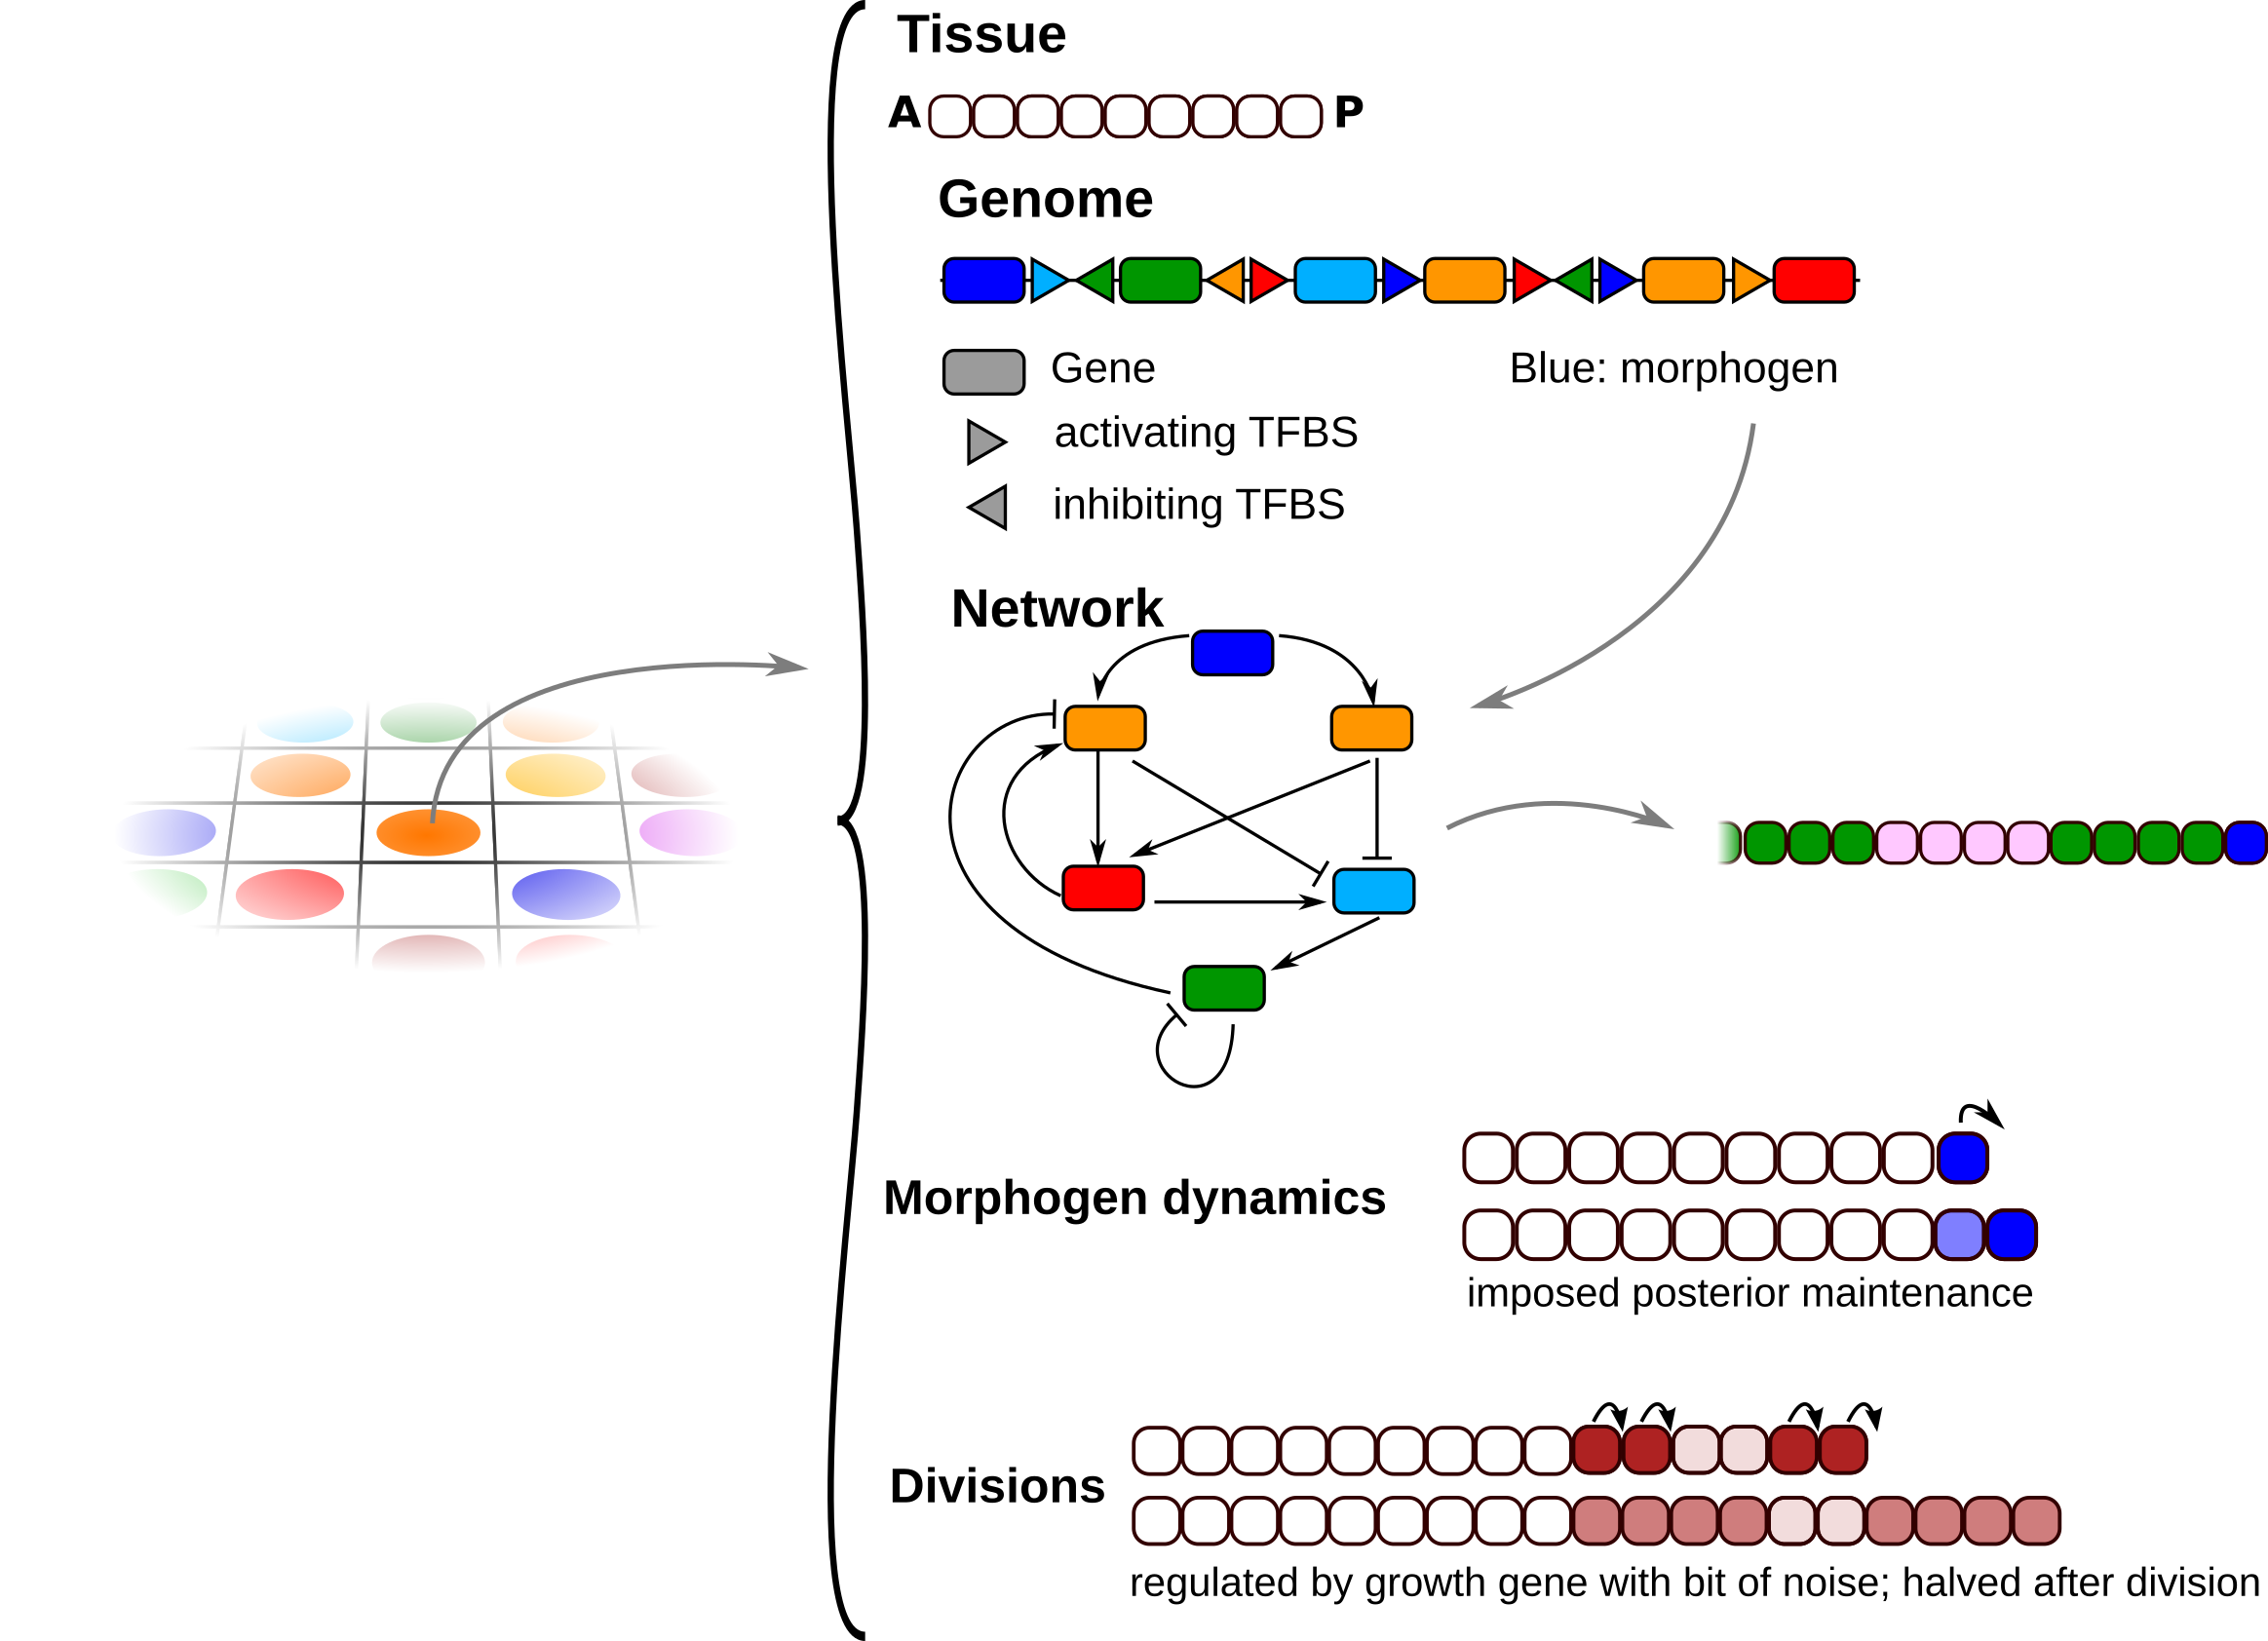
\includegraphics[width=0.9\textwidth]{figures/individual_growth.png}\\
    \end{center}
\end{frame}

%may want to skip this frame?
\begin{frame}
    \frametitle{Selection and mutation}
    \begin{center}
     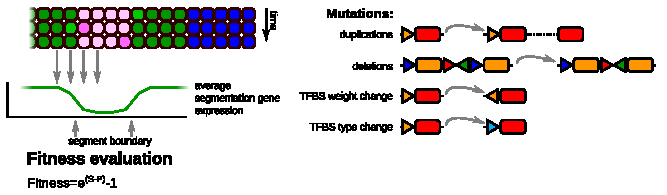
\includegraphics[width=1.\textwidth]{figures/fitness_mutations.pdf}\\
    \end{center}
\end{frame}

\begin{frame}
    \frametitle{Two main outcomes}
     \begin{center}
     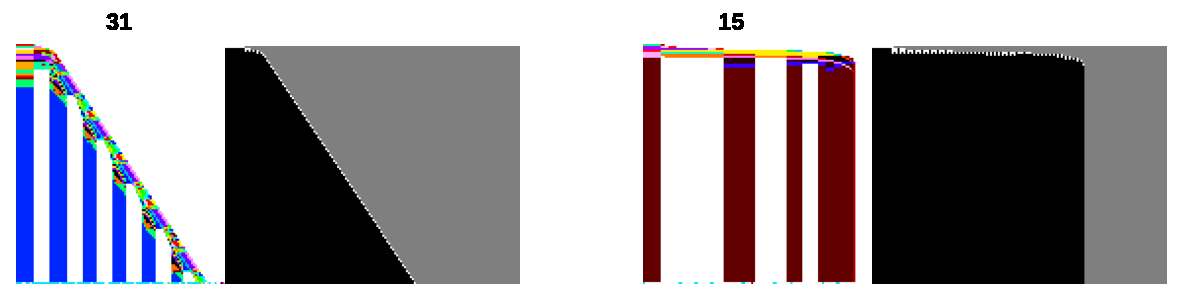
\includegraphics[width=1.\textwidth]{figures/two_strategies.pdf}\\
    \end{center}
    % seq. segmentation and simultaneous segmentation
    % seq segmentation is more robust and produces more segments
    % variations do evolve, and also some rare different mechanisms
\end{frame}

\begin{frame}
    \frametitle{Can evolution ``invent'' a morphogen gradient?}
    \begin{center}
     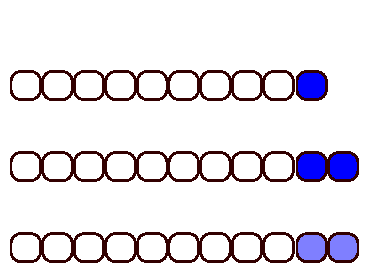
\includegraphics[width=0.6\textwidth]{figures/freemorph_initial.pdf}\\
    \end{center}
\end{frame}

\begin{frame}
    \frametitle{Prior presence of a morphogen gradient is essential}
    \begin{center}
     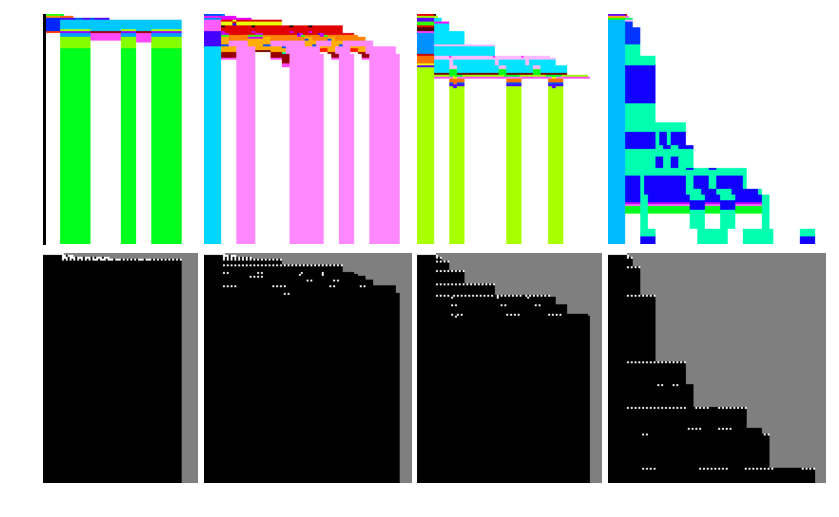
\includegraphics[width=0.9\textwidth]{figures/simultaneous_freemorph.pdf}\\
    \end{center}
    Mechanism uses division noise to steer different fates - very nonrobust.
\end{frame}

\begin{frame}
    \frametitle{Selection for stopping growth should come later}
    \begin{center}
     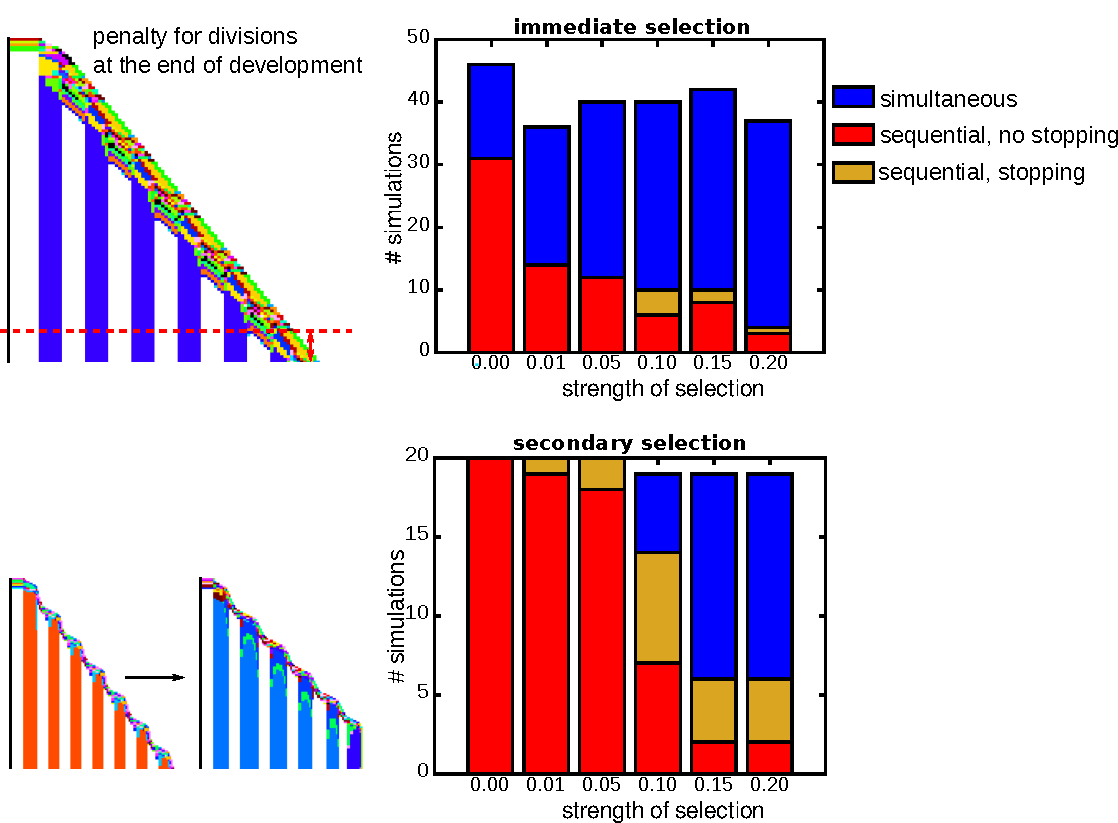
\includegraphics[width=.9\textwidth]{figures/stopgrowth_start.pdf}\\
    \end{center}
    % if we impose selection for determinate growth immediately, lose seq. solutions
    % slightly better if secondarily selected
\end{frame}

\begin{frame}
    \frametitle{Conclusions}
    Posterior morphogen: posterior growth \& sequential segmentation\\
    Determinate growth only after evolution of A-P growth\\
    \begin{center}
     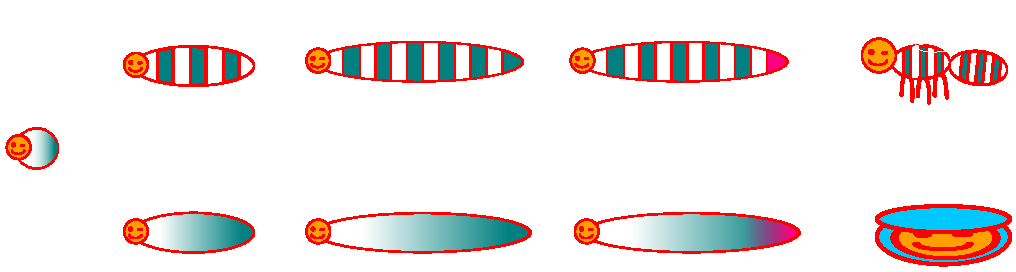
\includegraphics[width=1.\textwidth]{figures/conclusions.pdf}\\
    \end{center}
\end{frame}

\section{CPM in EvoDevo}
\begin{frame}
\frametitle{Studying the evolution of side effects}   
\begin{center}
     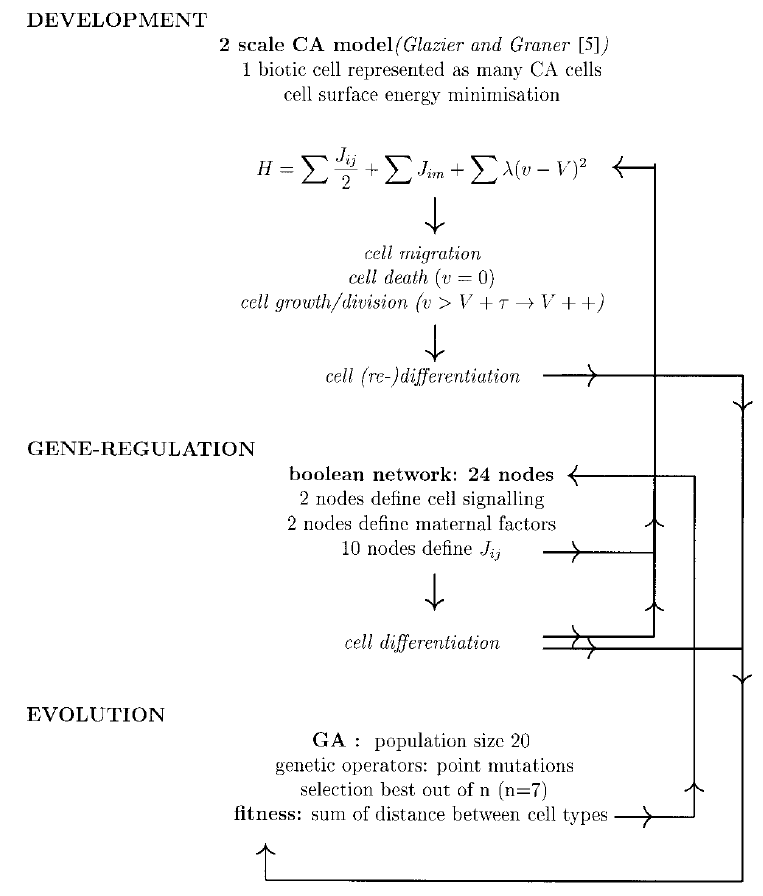
\includegraphics[width=0.6\textwidth]{figures/hogeweg_model.png}\\
    \end{center}
\end{frame}

\begin{frame}
\frametitle{First few cleavages are programmed}   
\begin{center}
     
\includegraphics[width=0.8\textwidth]{figures/hogeweg_model2.pdf}\\
    \end{center}
\end{frame}


\begin{frame}
\frametitle{Studying the evolution of side effects}   
\begin{center}
     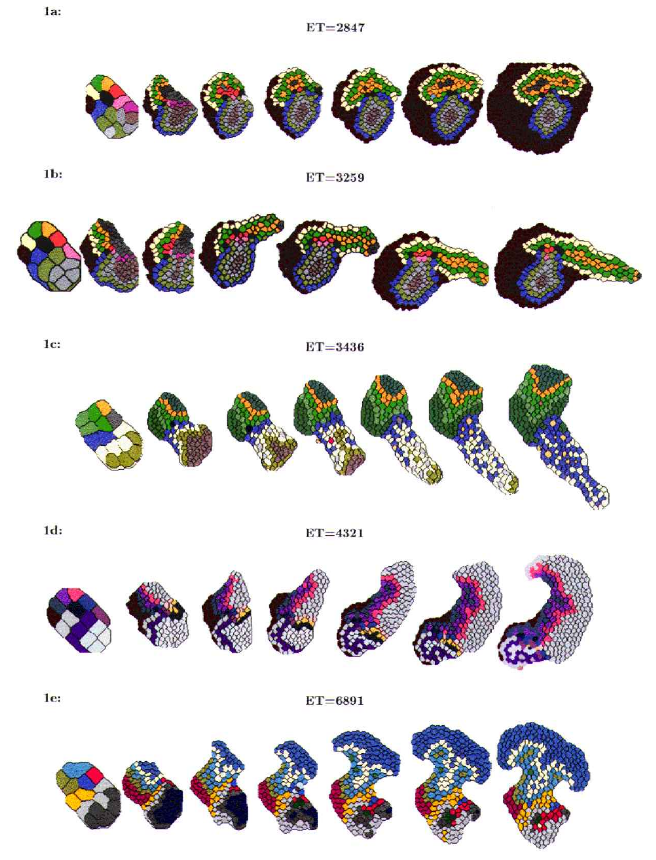
\includegraphics[width=0.5\textwidth]{figures/hogeweg_dev.png}\\
    \end{center}
\end{frame}


\begin{frame}
\frametitle{Studying the evolution of side effects}   
\begin{center}
     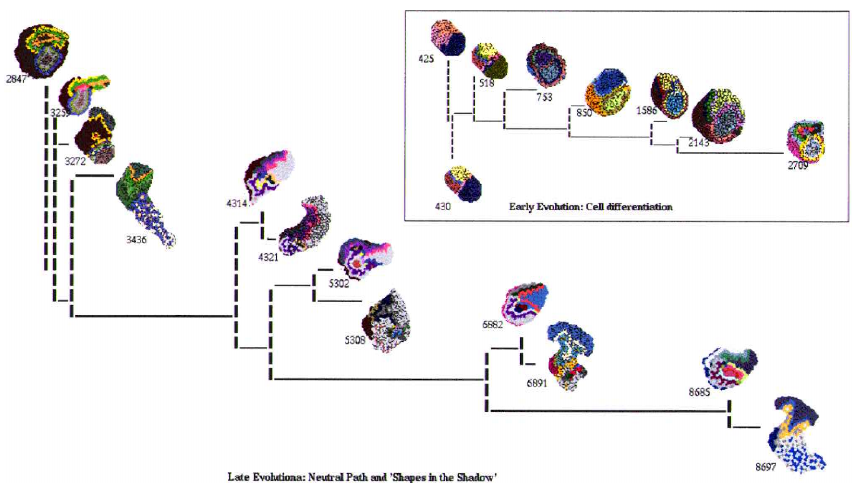
\includegraphics[width=0.9\textwidth]{figures/hogeweg_shadow.png}\\
    \end{center}
\end{frame}

\begin{frame}
\frametitle{Studying the evolution of side effects}   
\begin{center}
     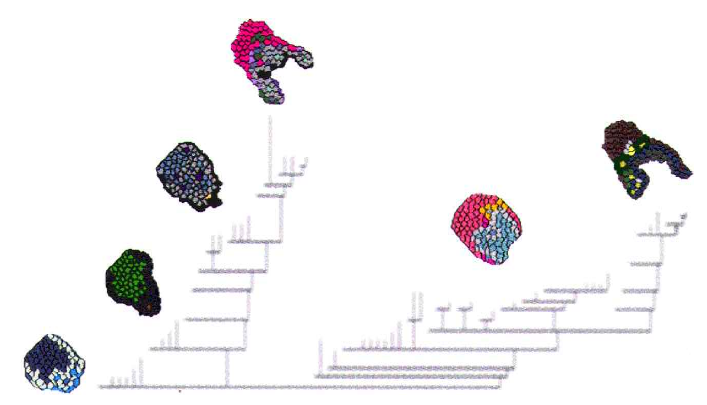
\includegraphics[width=0.9\textwidth]{figures/hogeweg_replaytape.png}\\
    \end{center}
\end{frame}

\section{Wrapping up}

\begin{frame}
\frametitle{Models at different levels}   
\begin{center}
     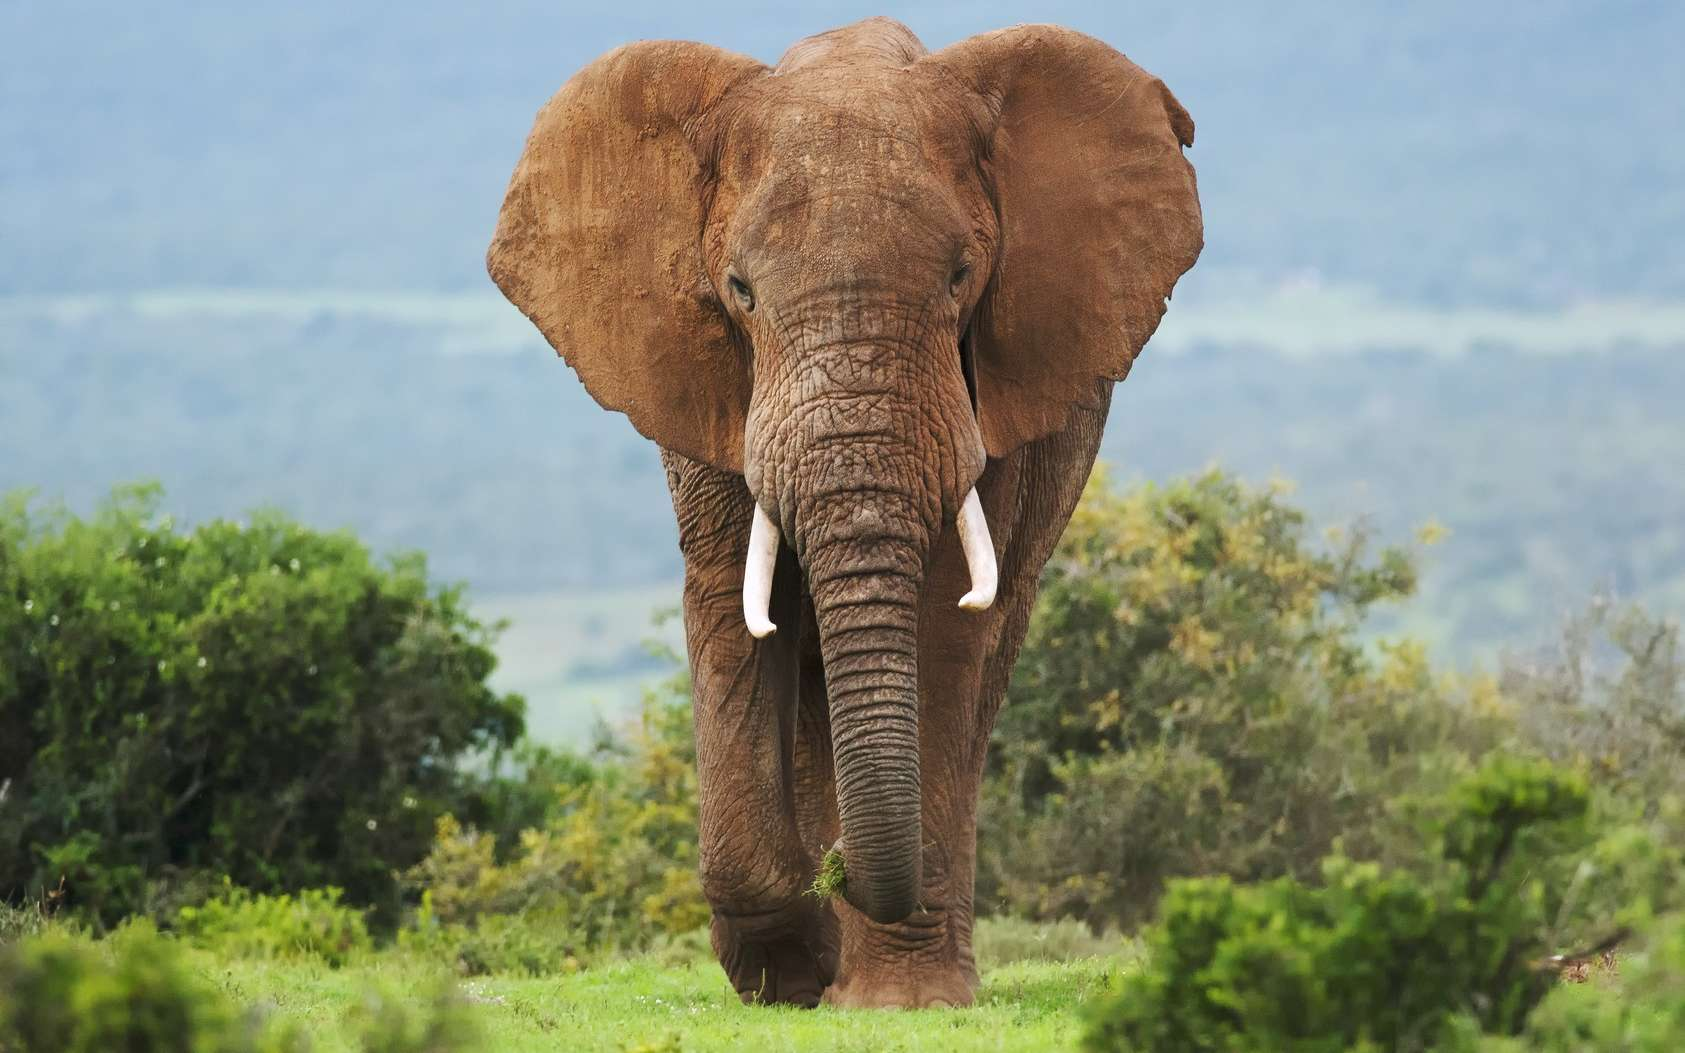
\includegraphics[width=0.7\textwidth]{figures/elephant.jpg}\\
    \end{center}
\end{frame}

\end{document}

